\documentclass{beamer}
\usetheme{metropolis}

\usepackage{graphicx}
\graphicspath{{images/}}

\DeclareMathOperator{\cdf}{cdf}
\DeclareMathOperator{\disc}{disc}
\DeclareMathOperator{\ST}{ST}
\newcommand{\bC}{\mathbf{C}}
\newcommand{\bF}{\mathbf{F}}
\newcommand{\bZ}{\mathbf{Z}}
\newcommand{\dd}{\mathrm{d}}

\title{Equidistribution, discrepancy, and the analytic properties of Dirichlet series}
\author{Daniel Miller}
\institute{Cornell University}
\date{27 November 2016}





\begin{document}

\begin{frame}
\titlepage
\end{frame}

\begin{frame}
\frametitle{Outline}
\tableofcontents
\end{frame}

\section{Background}

\begin{frame}{Elliptic curves}
Equation of the form $E:y^2=x^3+ax+b$.
\pause

Simplify: assume $a,b\in \bZ$.
\pause

Non-singular: $4a^3+27b^2\ne 0$. 
\pause

Count points modulo $p$: 
\[
	\# E(\bF_p) = \#\{(x,y)\in (\bF_p)^2 : x^2=y^3+ax+b\} + 1 .
\]
\pause

$+1=$ ``point at infinity.''
\pause

Geometric structure of $E(\bC)$
\end{frame}

\begin{frame}{Our example}
\begin{center}
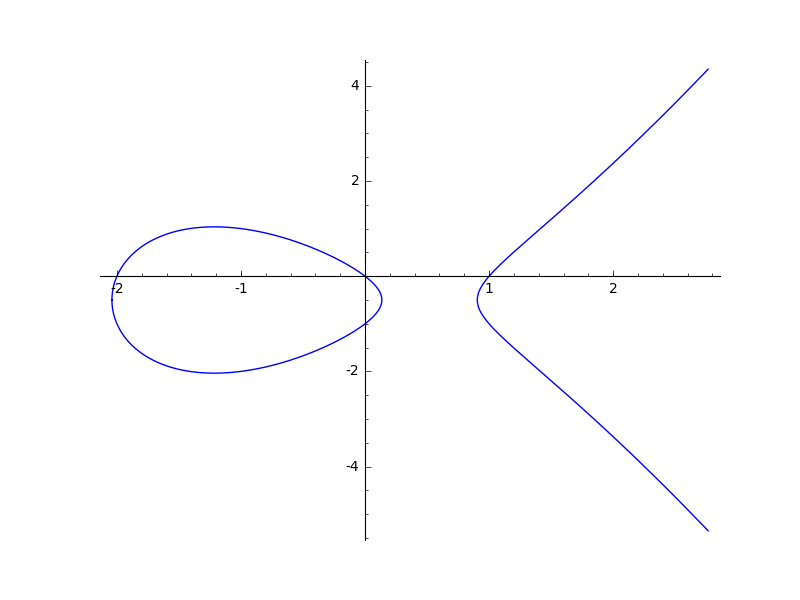
\includegraphics[width=0.7\textwidth]{rank2_contour}

$E:y^2+y = x^3+x^2-2x$
\end{center}
\pause

Where is $\infty$?
\end{frame}

\begin{frame}{Initial data}
\begin{tabular}{c|ccccccccc}
$p$ & 2 & 3 & 5 & 7 & 11 & 13 & \ldots & 999999929 & 999999937 \\ \hline
$\# E(\bF_p)$ & 1 & 2 & 3 & 3 & 8 & 11 & \ldots & 999950222 & 1000031072
\end{tabular}

\pause
Look at more data\ldots
\end{frame}

\begin{frame}
\begin{center}
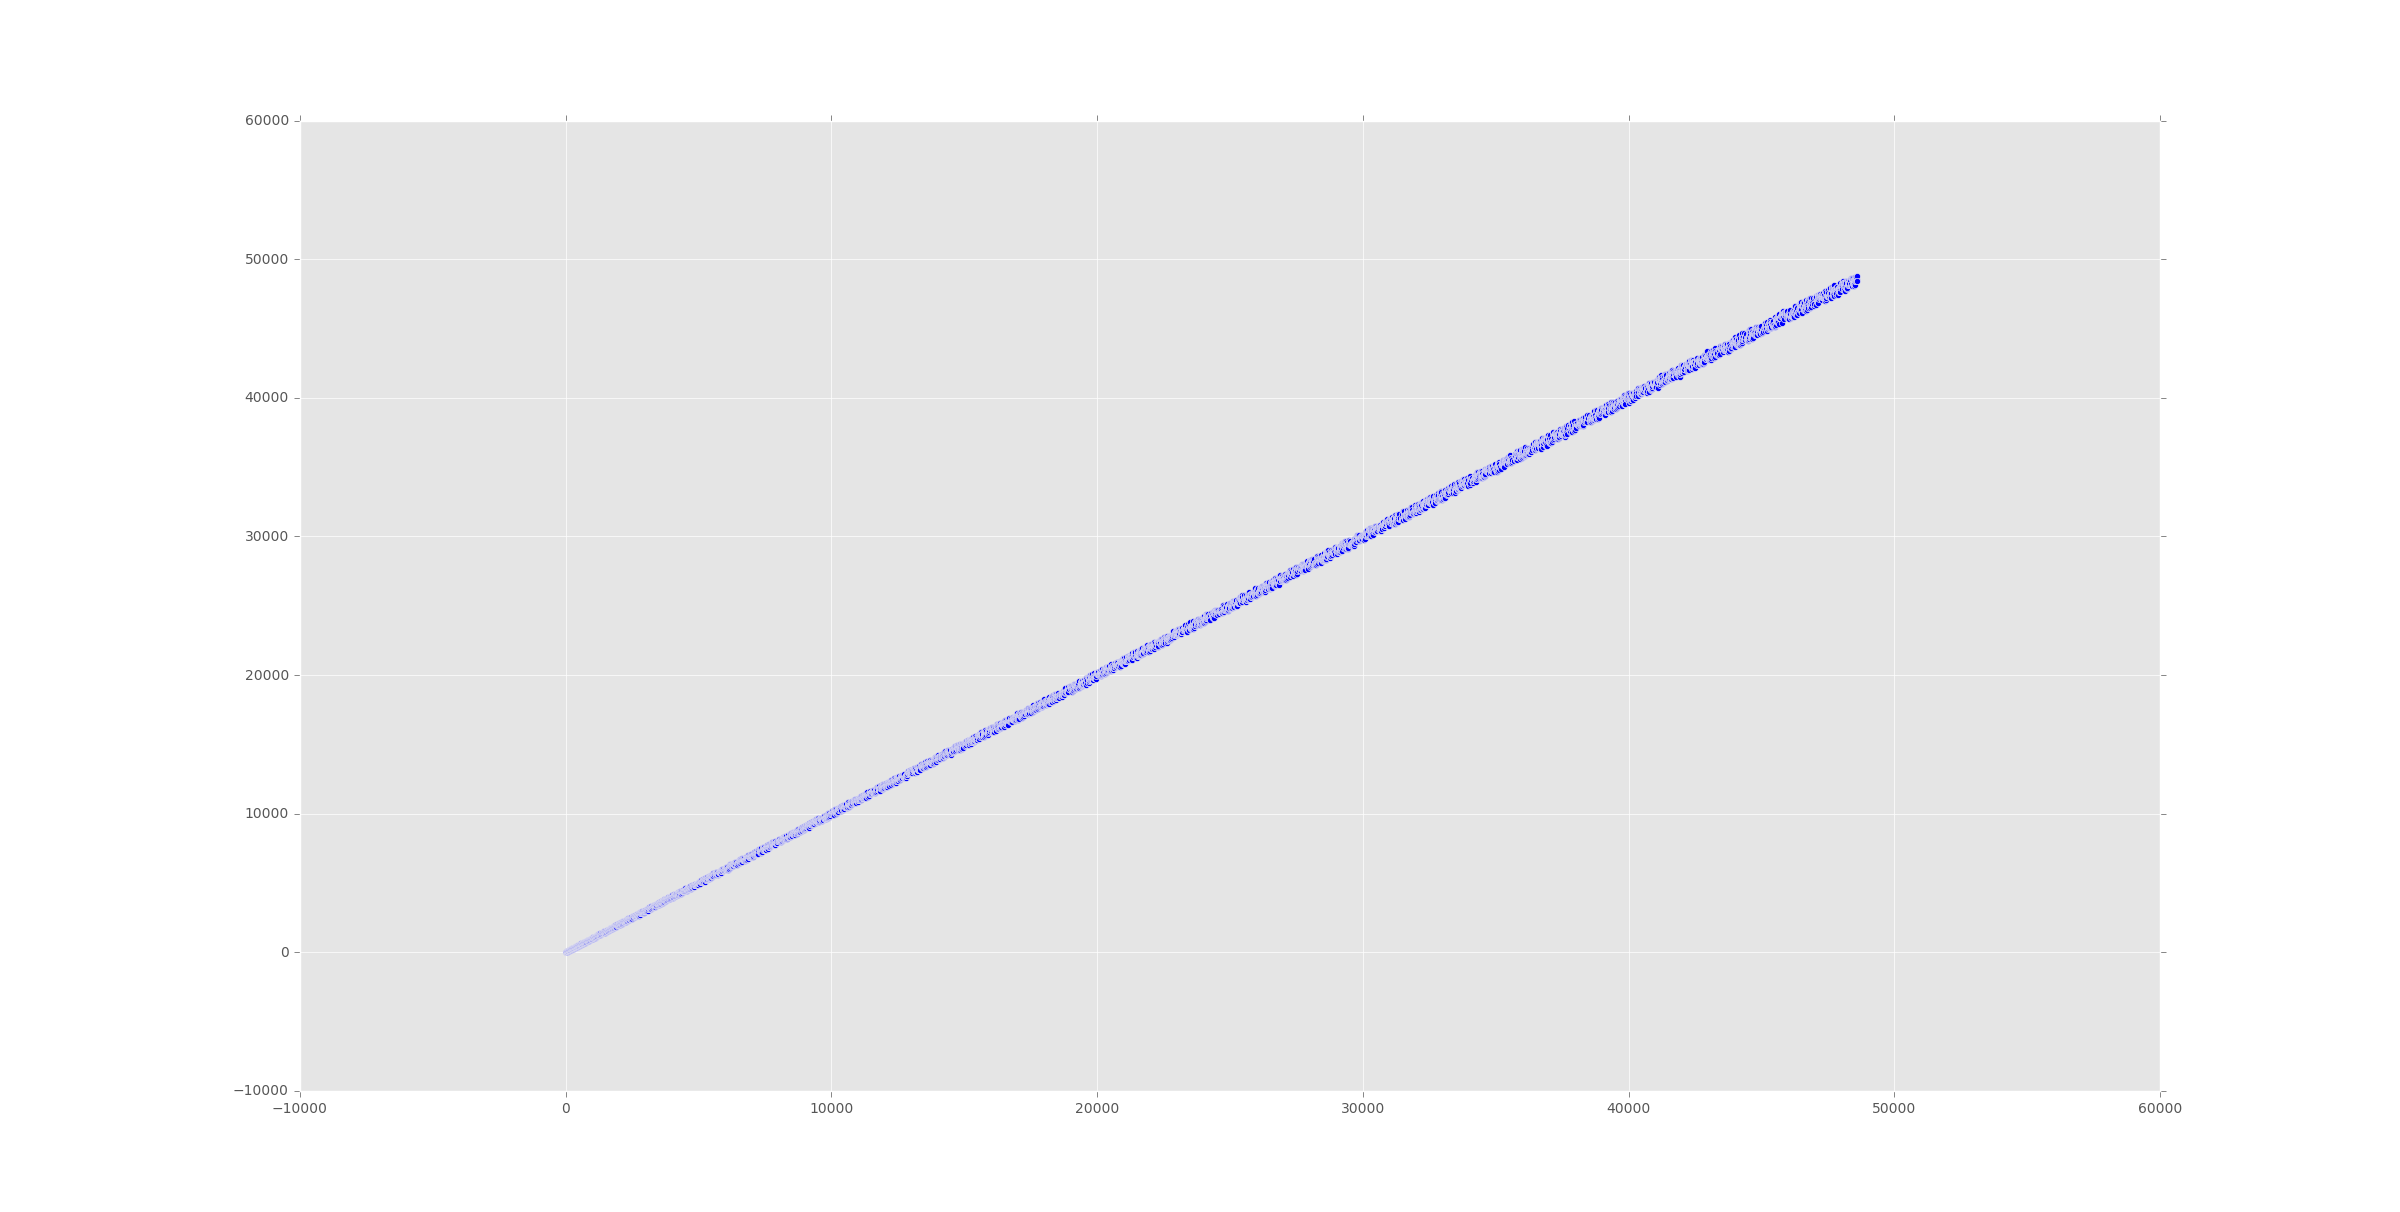
\includegraphics[width=\textwidth]{rank2_point_counts}

$\# E(\bF_p)$ as a function of $p$.
\end{center}
\pause

How does the error term behave?
\end{frame}

\begin{frame}{Hasse bound}
\begin{center}
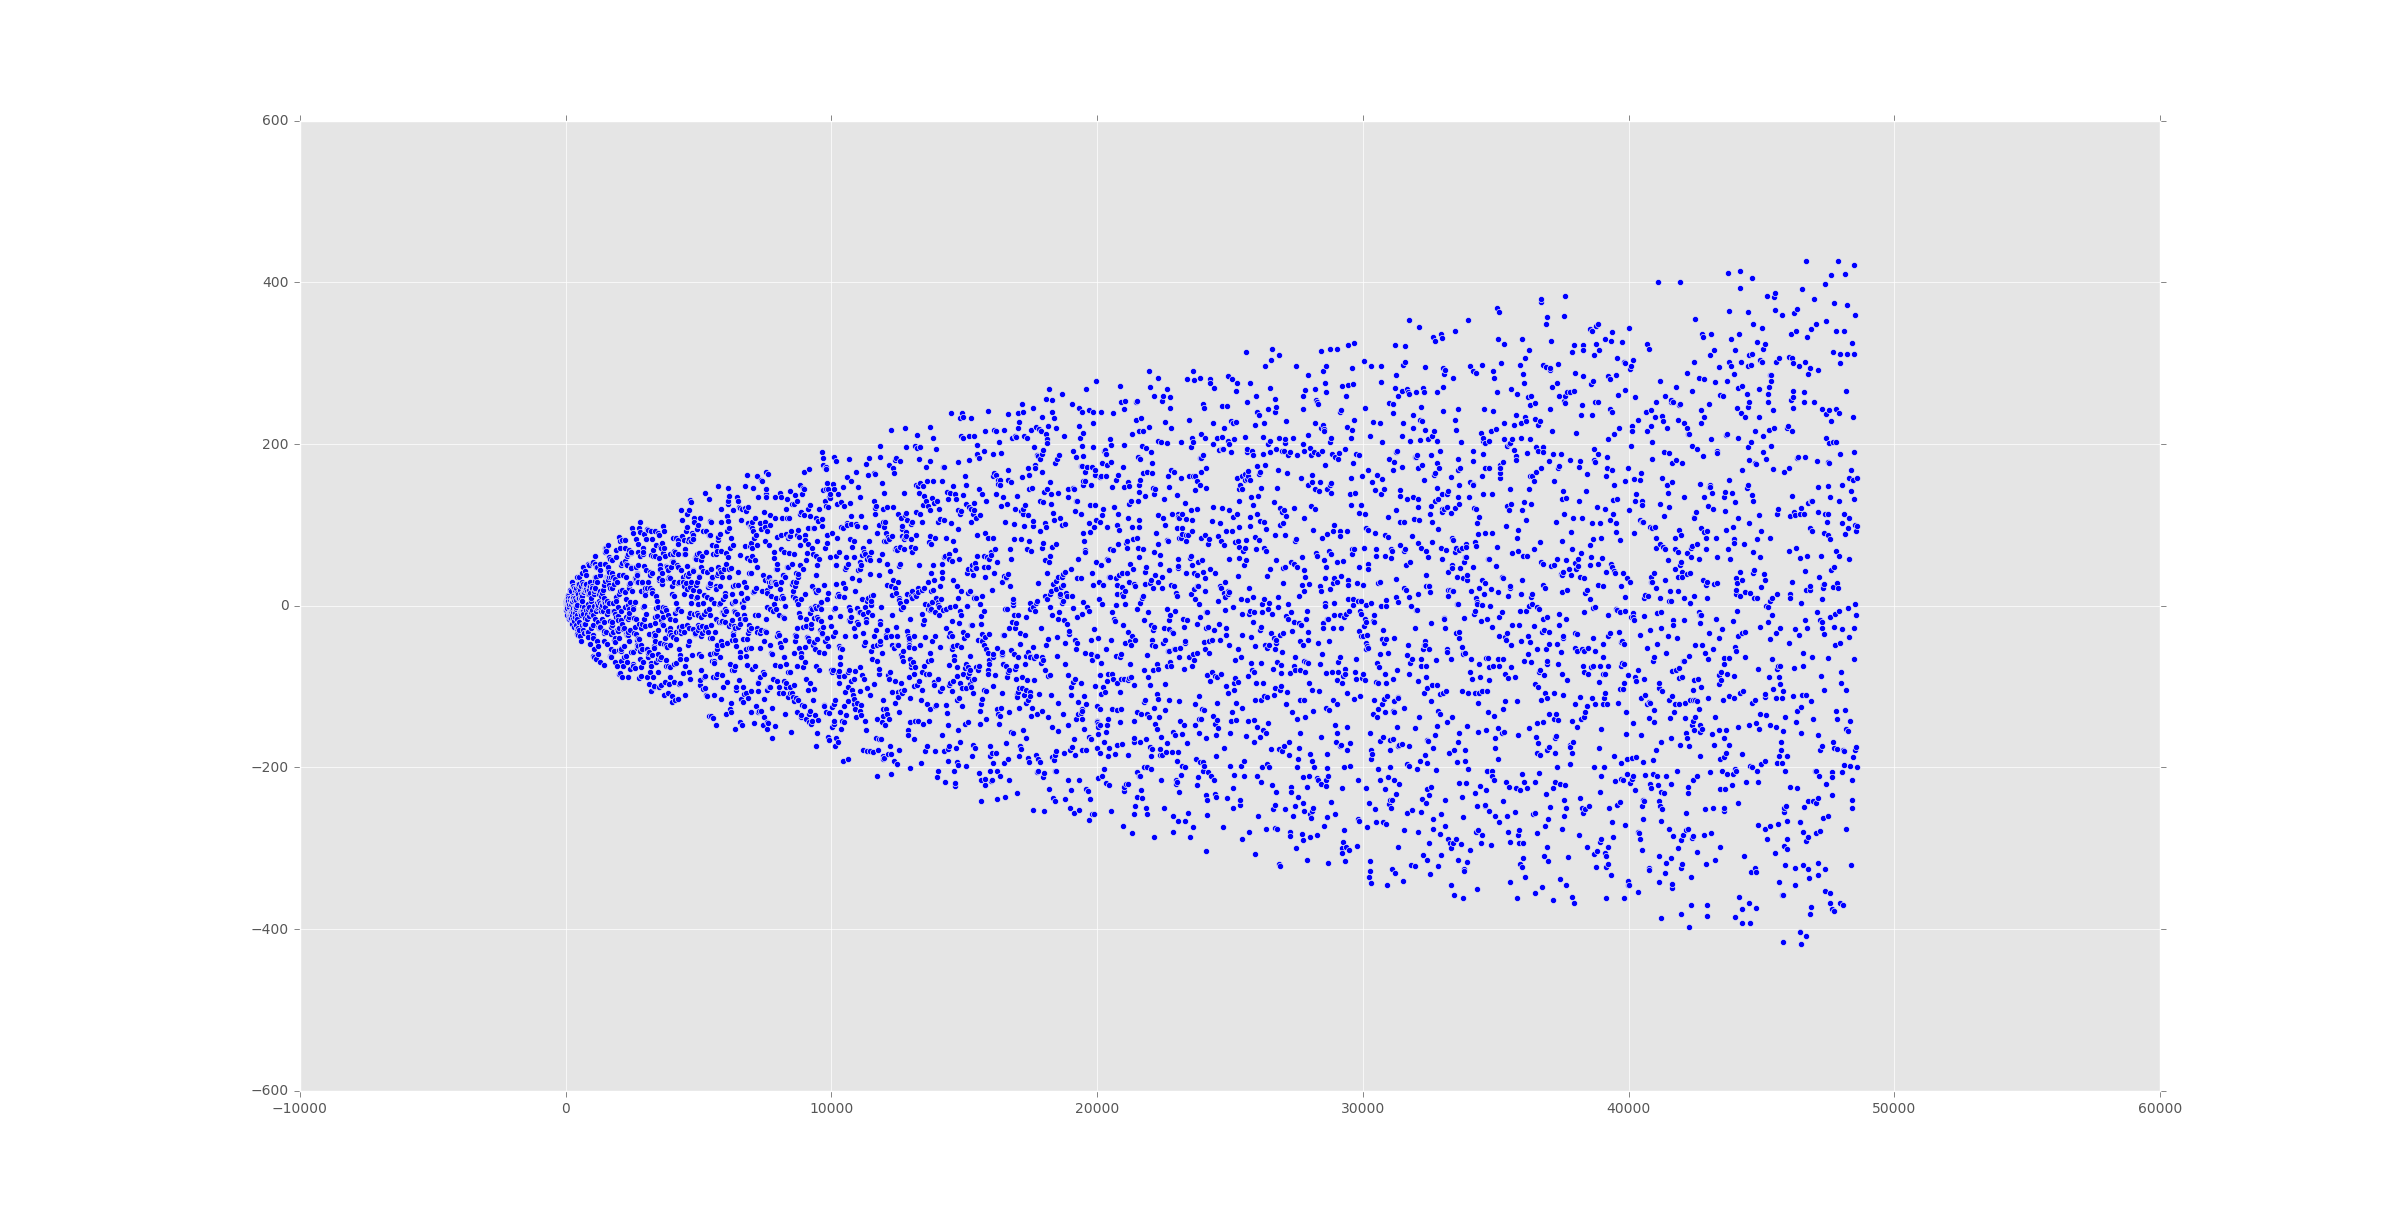
\includegraphics[width=\textwidth]{rank2_trace_Frobenius}

$a_p(E):=p+1-\# E(\bF_p)$ as a function of $p$.
\end{center}

\pause
Intuition: why is $a_p$ small? (and how small is it?)
\end{frame}

\begin{frame}{Hasse bound}
\begin{center}
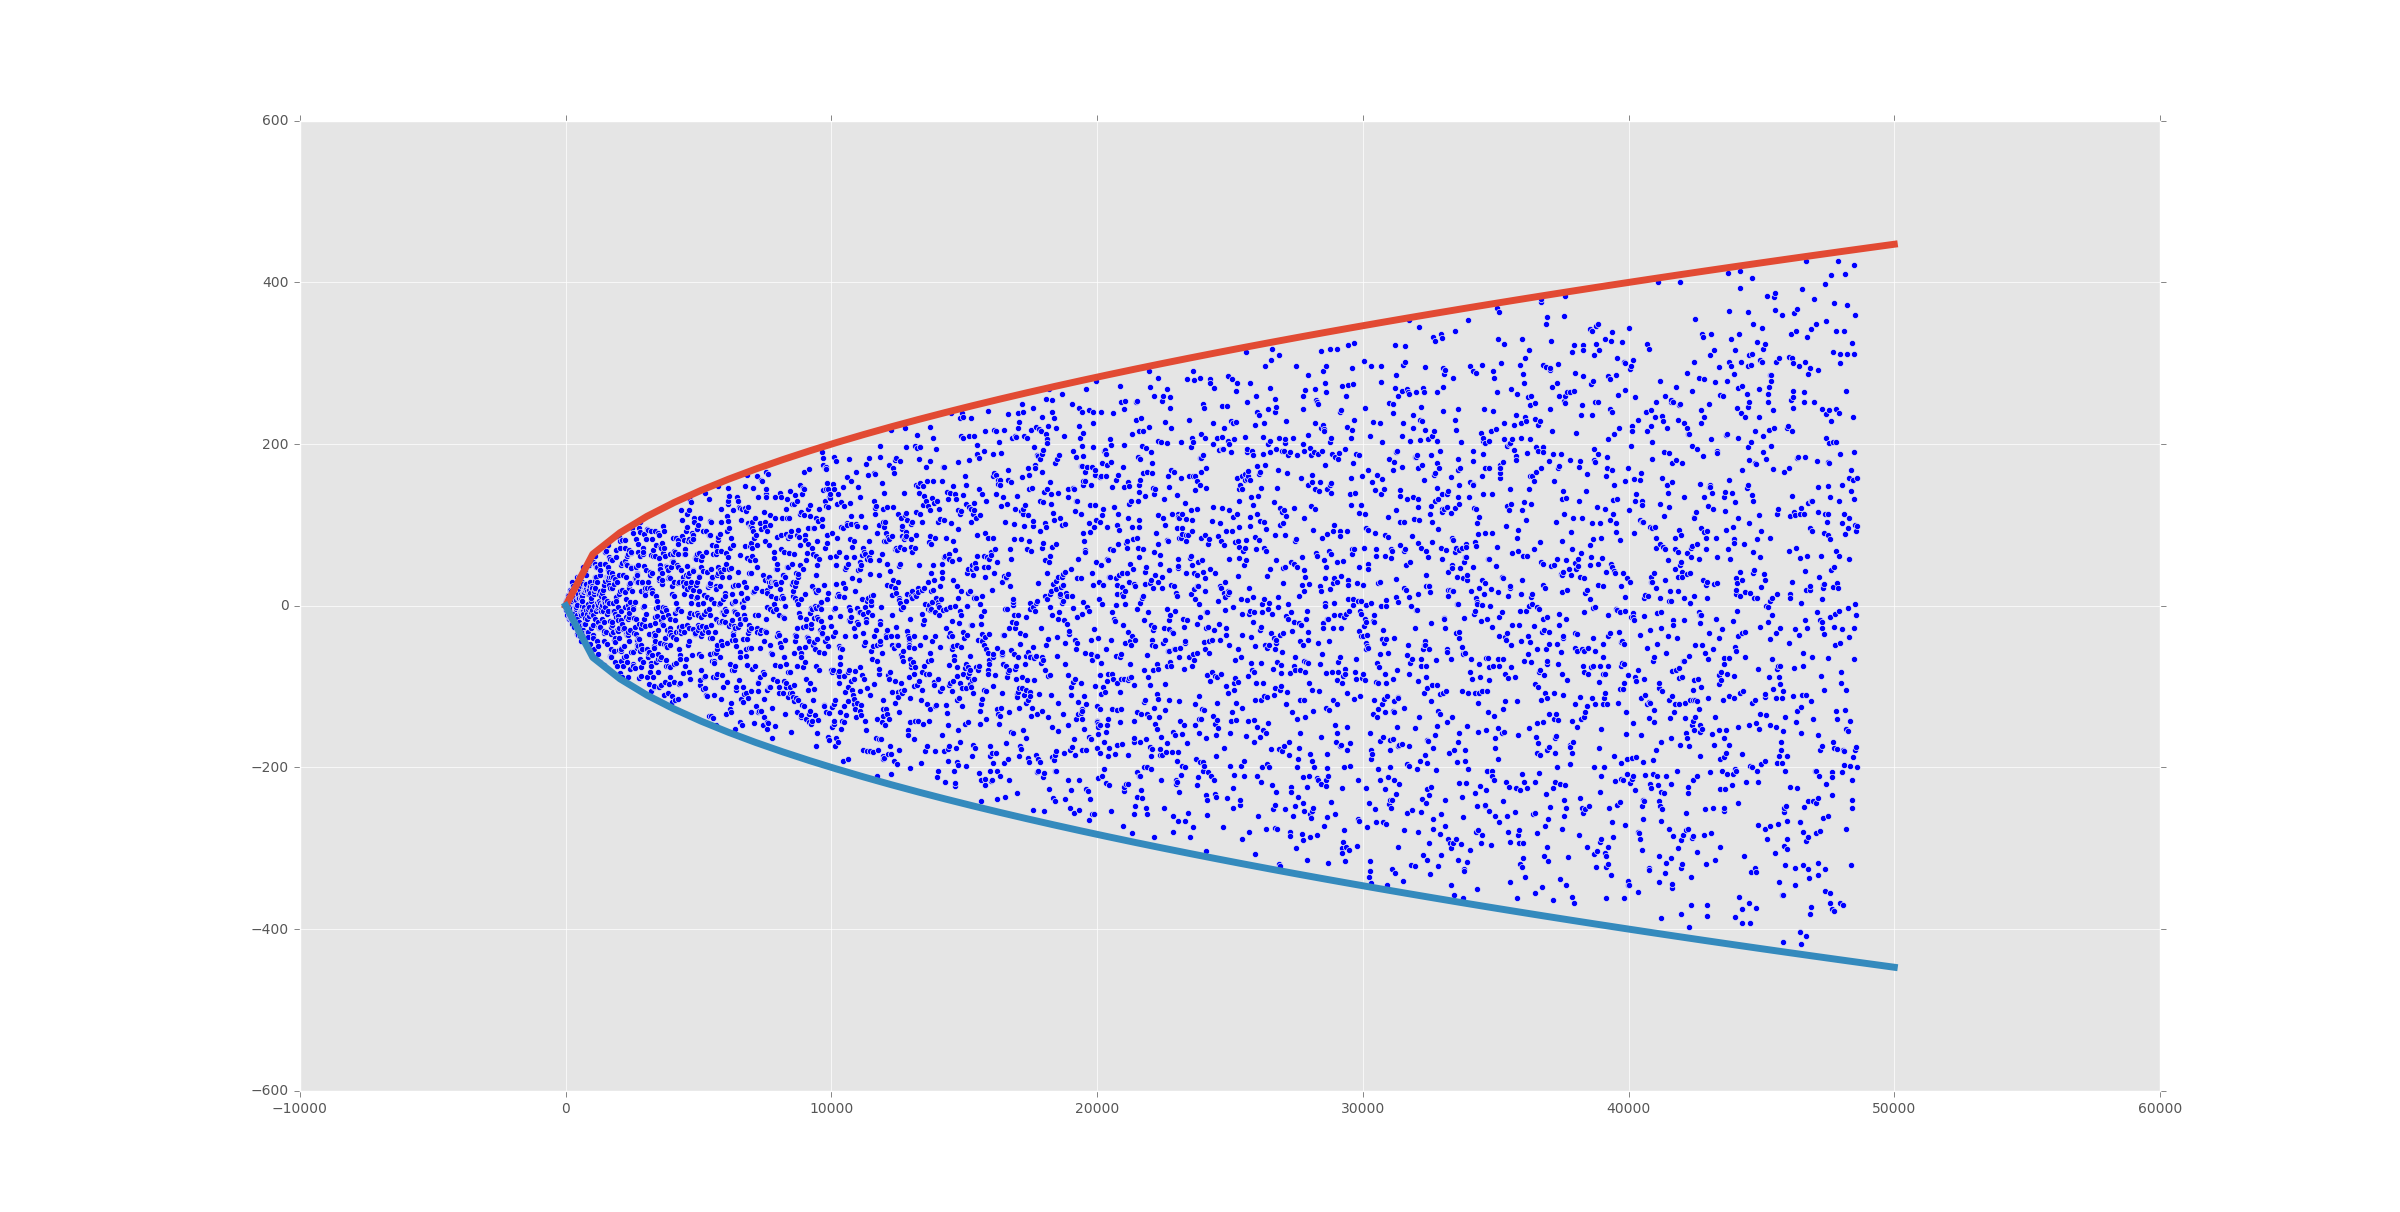
\includegraphics[width=\textwidth]{rank2_Hasse}

$a_p(E)$ vs.~$\pm 2\sqrt p$.
\end{center}

\pause
Perhaps we should normalize?
\end{frame}

\begin{frame}{Satake parameters}
\begin{center}
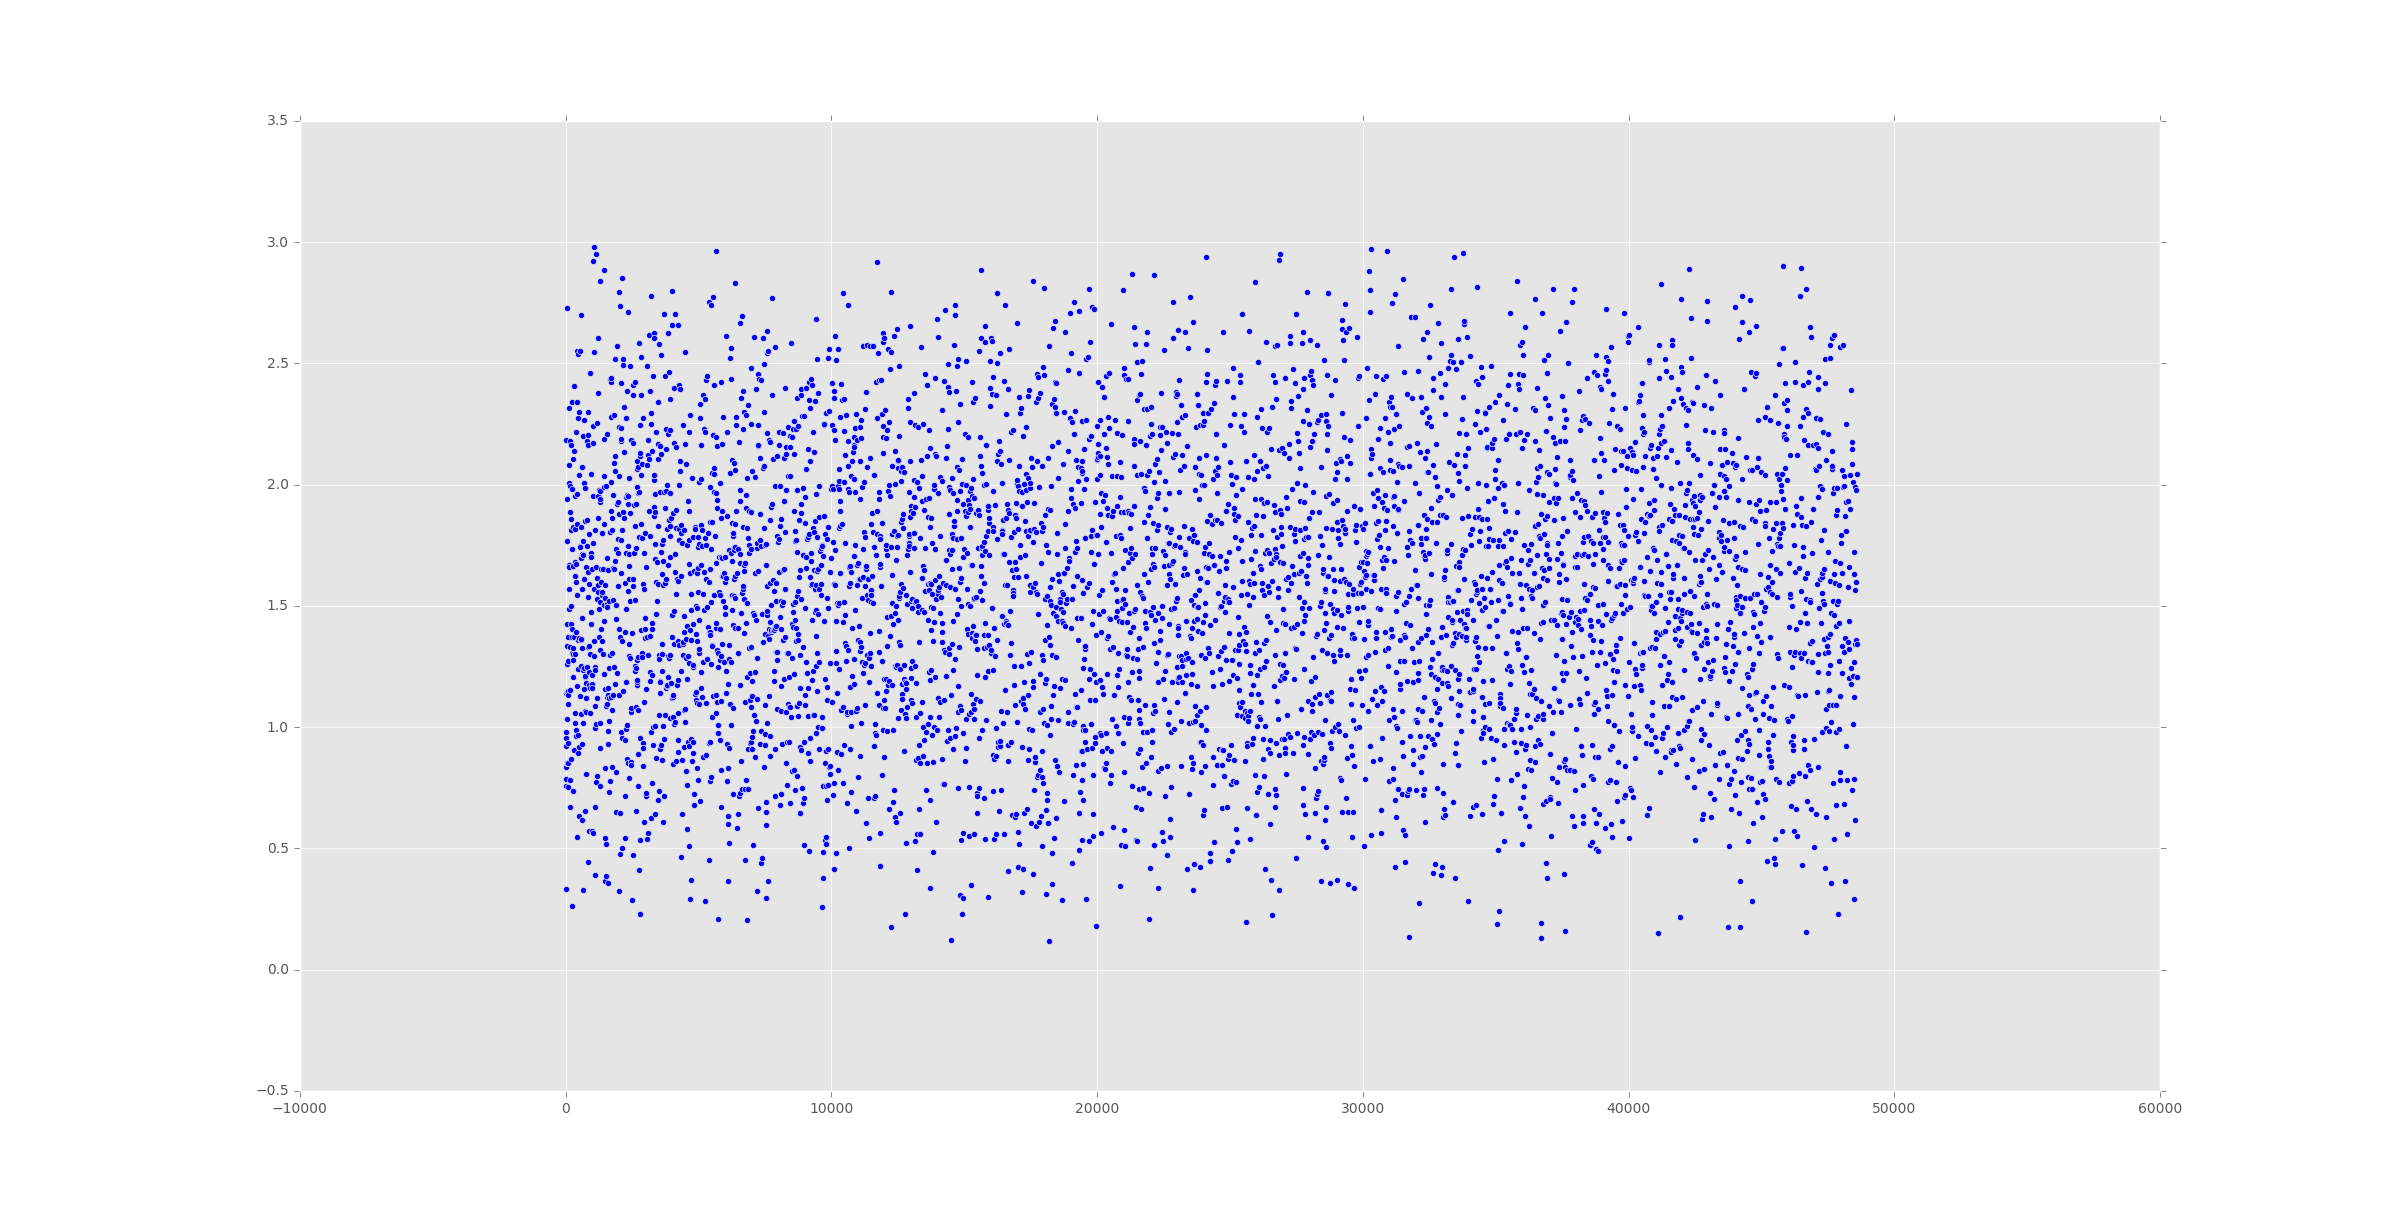
\includegraphics[width=\textwidth]{rank2_Satake}

$\theta_p = \cos^{-1}\left(\frac{a_p}{2\sqrt p}\right)$ as a function of $p$.
\end{center}

\pause
Look at the statistics of $\{\theta_p\}$. 
\end{frame}

\begin{frame}{Their statistics}
\begin{center}
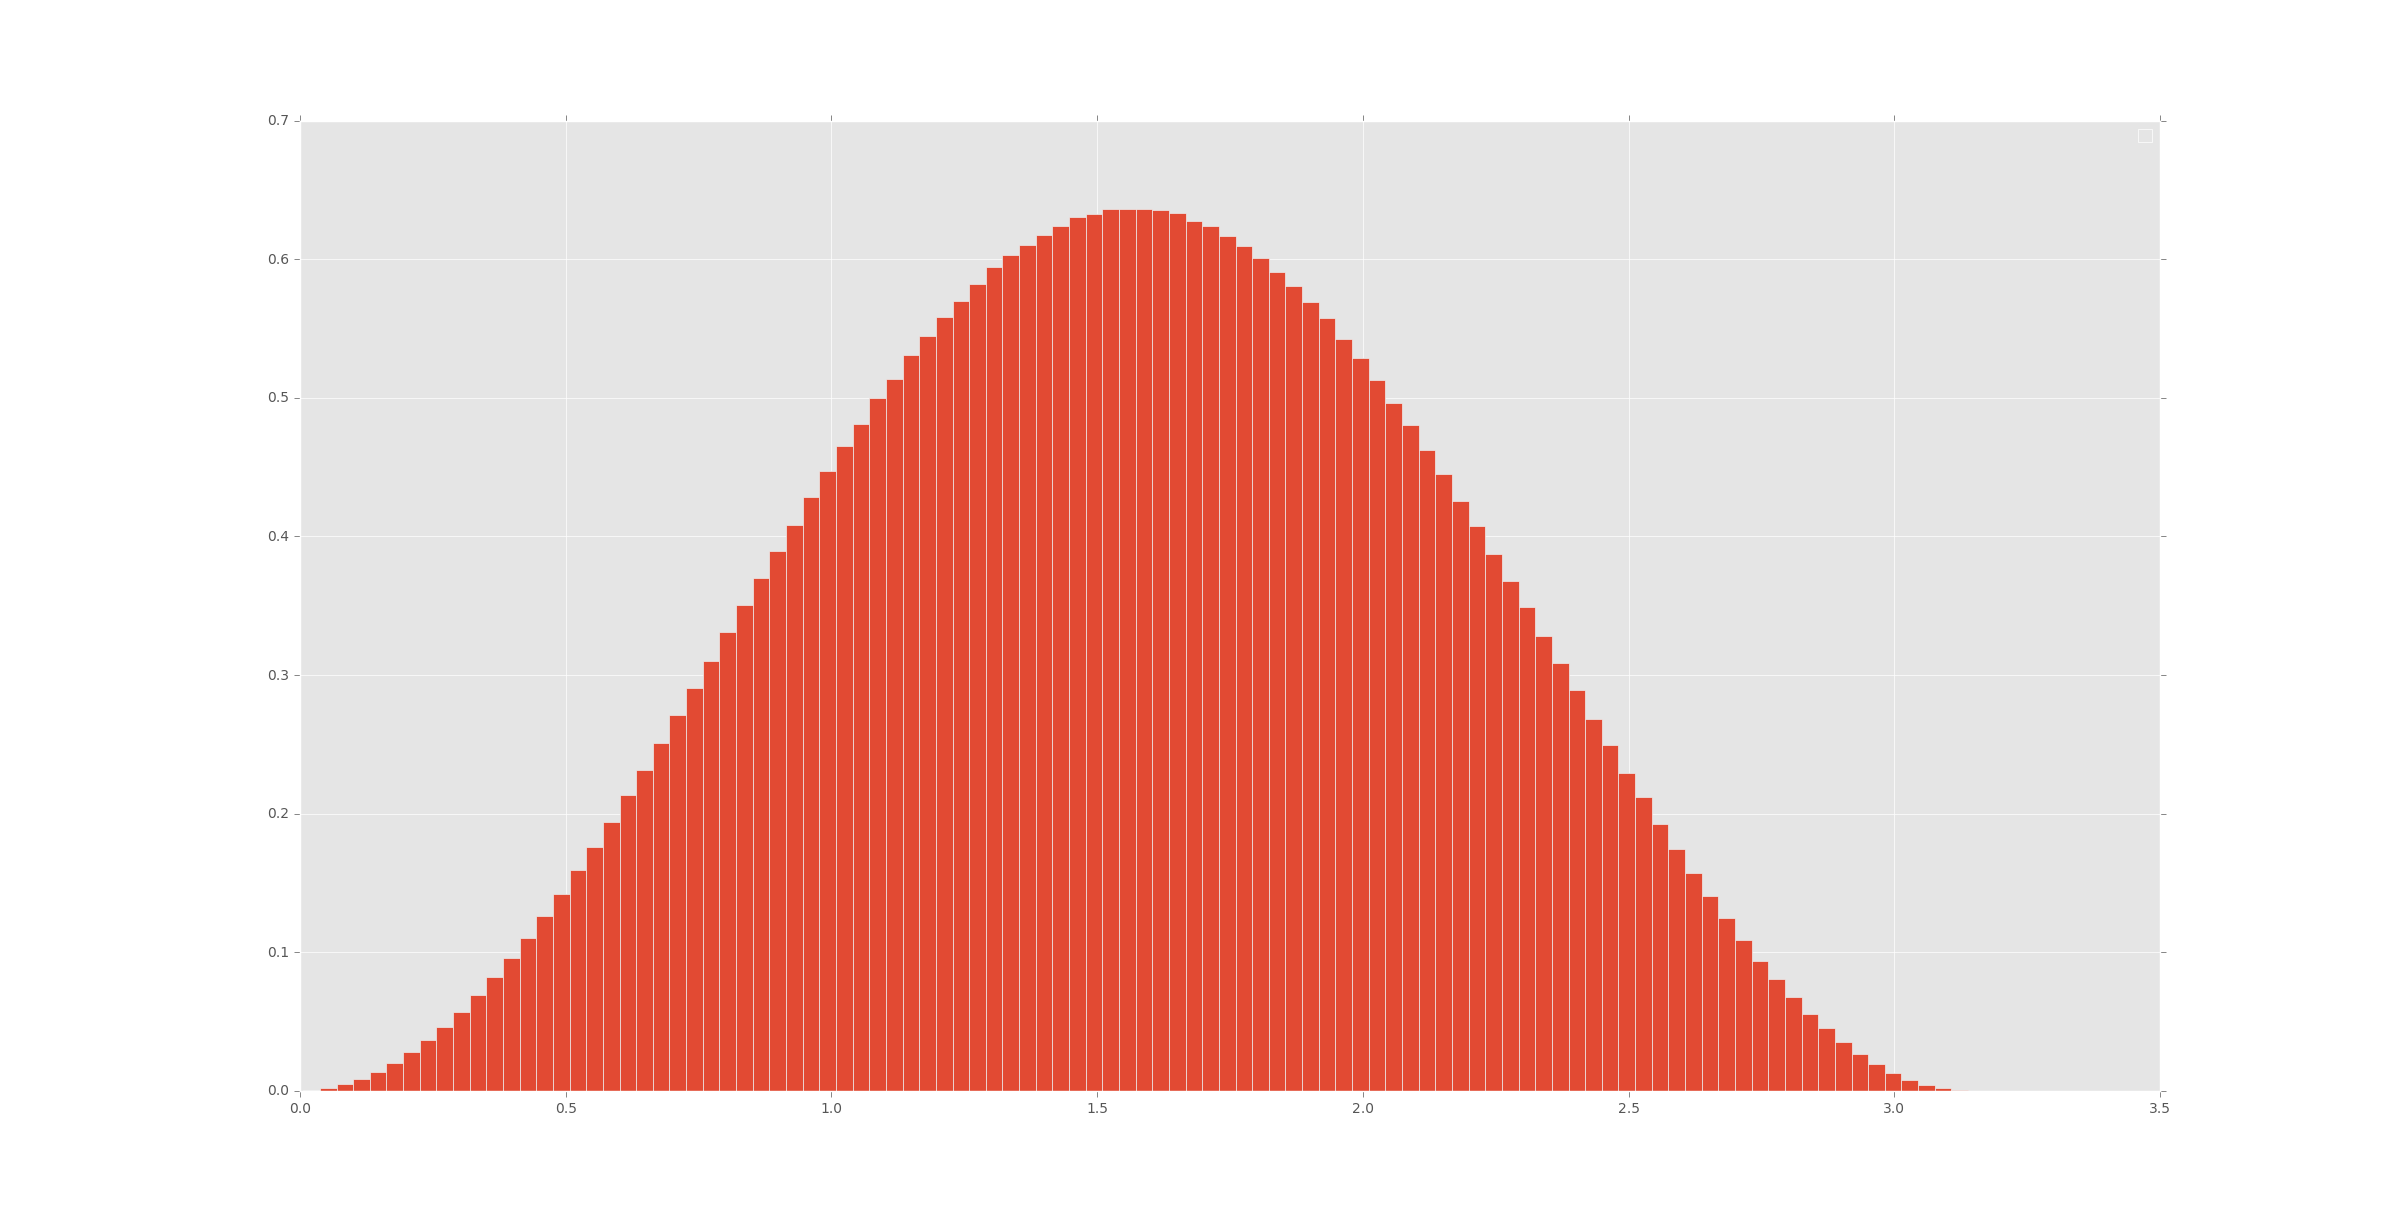
\includegraphics[width=\textwidth]{hist}

Histogram of $\{\theta_p\}_{p\leqslant 10^9}$.
\end{center}
\end{frame}

\begin{frame}{Their statistics}
\begin{center}
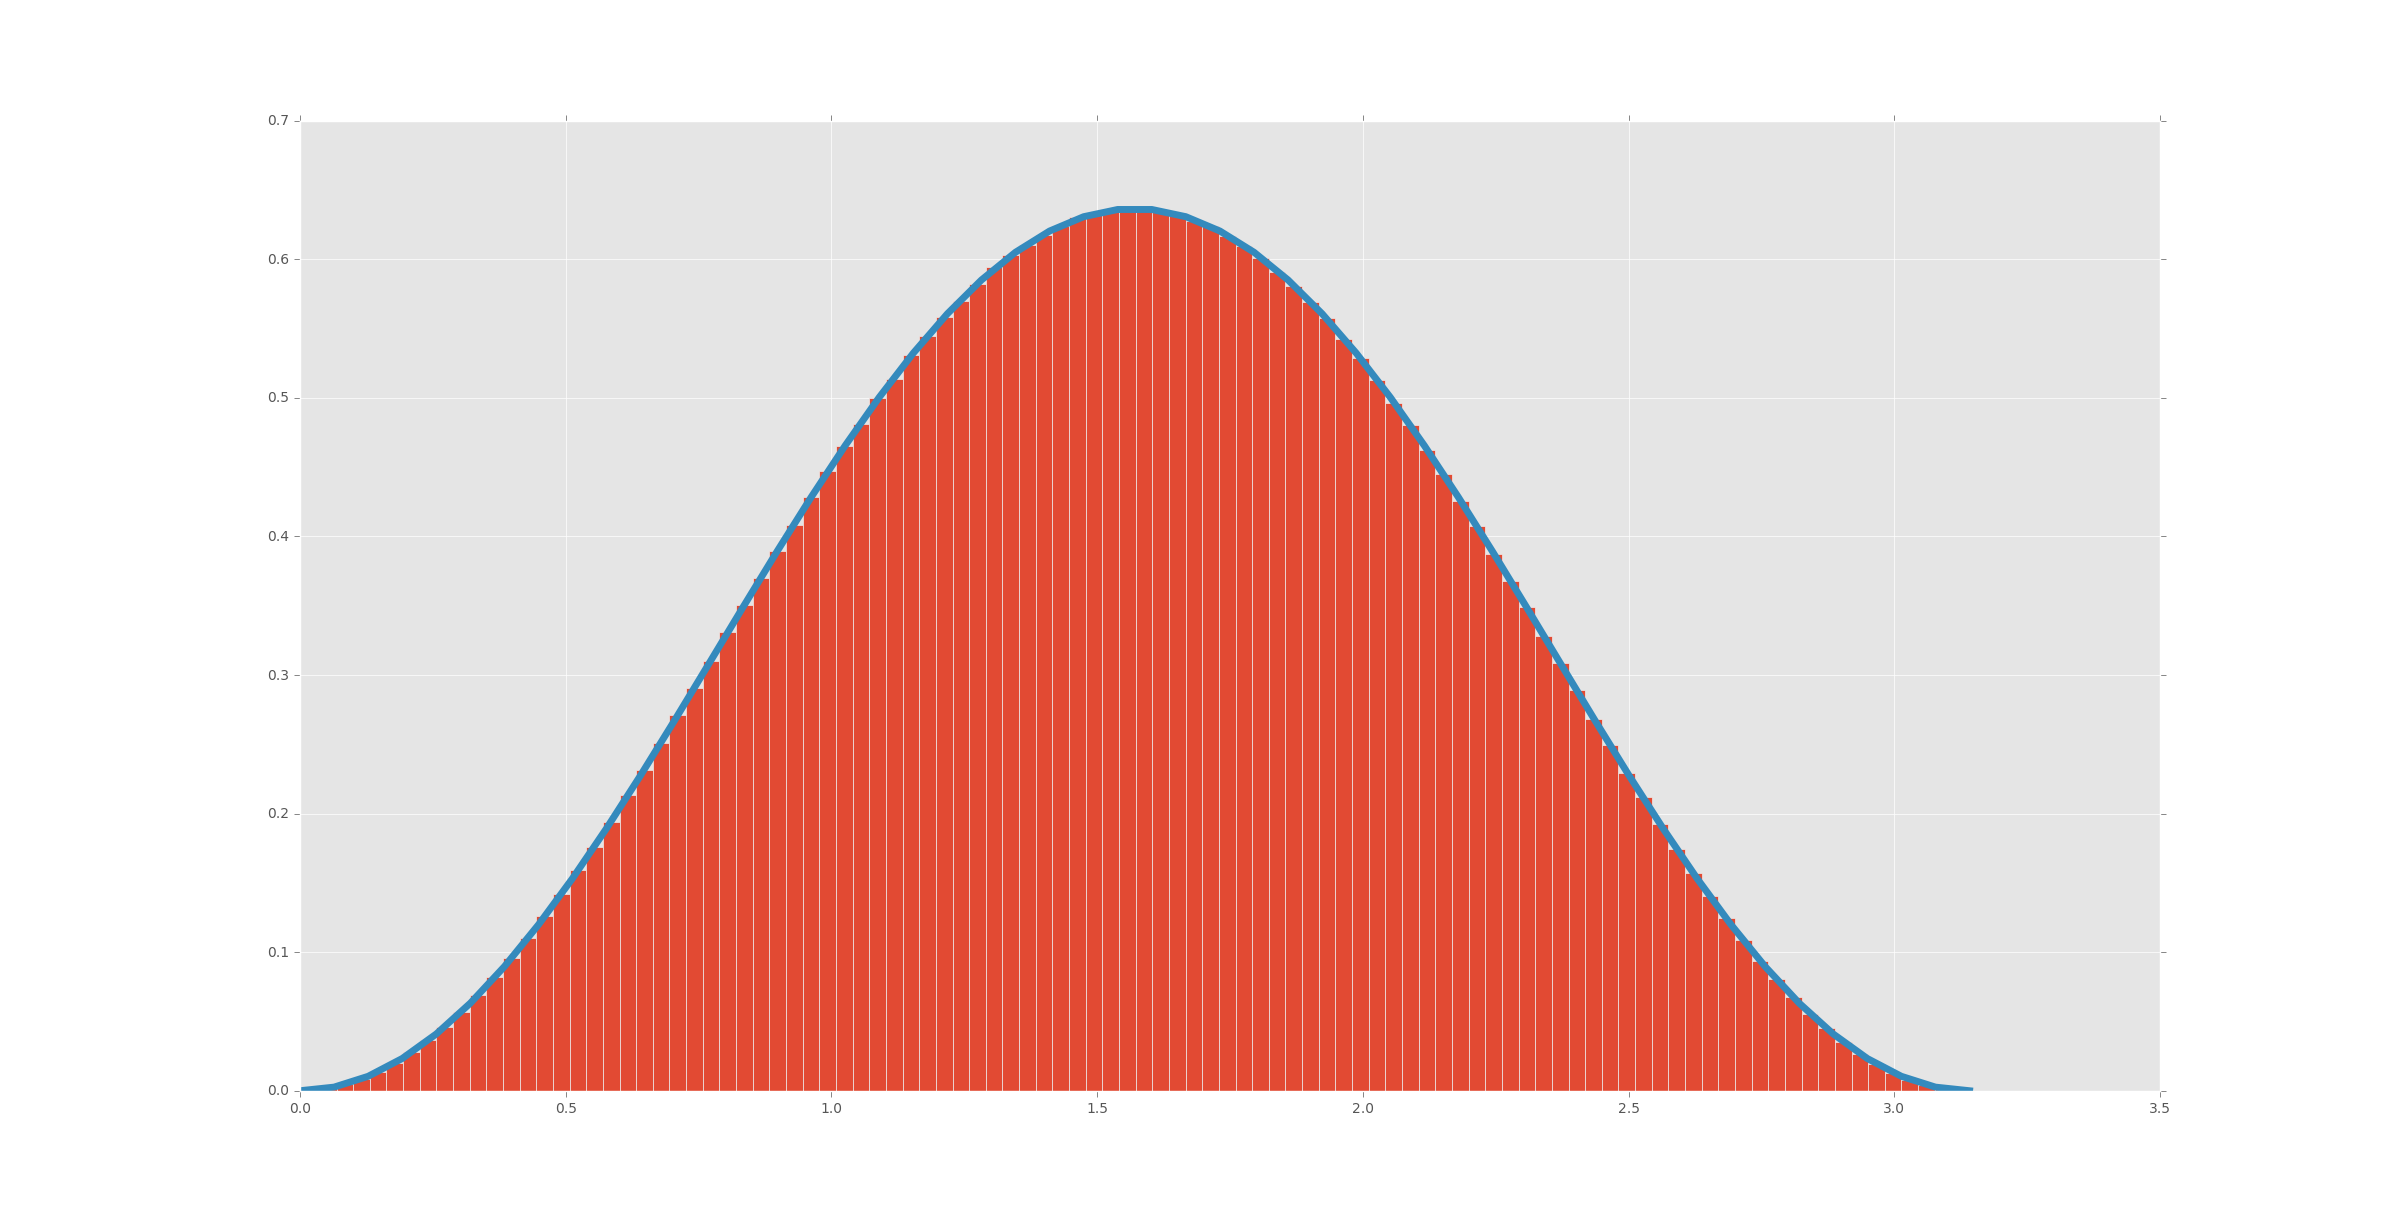
\includegraphics[width=\textwidth]{hist_with_density}

Histogram with graph of $\ST(\theta)=\frac{2}{\pi}\sin^2(\theta)$.
\end{center}

\pause
Some kind of convergence happening\ldots
\end{frame}

\section{The Sato--Tate conjecture}

\begin{frame}{Some definitions}
Two cumulative distribution functions:
\begin{align*}
	\cdf_N(x) &= \frac{\# \{p\leqslant N : \theta_p \leqslant x\}}{\#\{p\leqslant N\}} \\ 
	\cdf_{\ST}(x) &= \int_0^x \ST(x)\, \dd x = \frac{x-\sin(x)\cos(x)}{\pi} 
\end{align*}
\pause

Discrepancy
\begin{align*}
	\disc_E(N) = \sup_{0\leqslant x \leqslant \pi} |\cdf_N(x)-\cdf_{\ST}(x)| .
\end{align*}
\pause

Other ways to measure distabce between distributions?
\end{frame}


\begin{frame}{A deep theorem}
\begin{theorem}[Sato--Tate]
For any elliptic curve $E$, $\disc_E(N) \to 0$ as $N\to \infty$. 
\end{theorem}
\pause

\begin{block}{Conjecture (Akiyama--Tanigawa)}
For any elliptic curve $E$, $\disc_E(N) = O_E(N^{-\frac 1 2+\epsilon})$.
\end{block}
\pause

\begin{theorem}
The Akiyama--Tanigawa conjecture implies the Riemann Hypothesis (for the 
elliptic curve). 
\end{theorem}
\pause

Key idea: Koksma--Hlawka inequality.
\end{frame}


\begin{frame}{Some $L$-functions}
\begin{definition}[Riemann zeta function]
\[
	\zeta(s) = \prod_p \frac{1}{1-p^{-s}} = \sum_{n\geqslant 1} \frac{1}{n^s}
\]
\end{definition}
\pause

\begin{definition}[$L$-function of elliptic curve]
\[
	L(E,s) = \prod_p \frac{1}{(1-e^{i\theta_p}p^{-s})(1-e^{-i\theta_p}p^{-s})}
\]
\end{definition}
\pause

\begin{definition}[strange Dirichlet series]
\[
	L_f(E,s) = \prod_p \frac{1}{1-f(\theta_p)p^{-s}}
\]
\end{definition}
\pause

(Standing assumption: $\int f\cdot \ST = 0$.)
\end{frame}


\begin{frame}{$L$-functions on the complex plane}
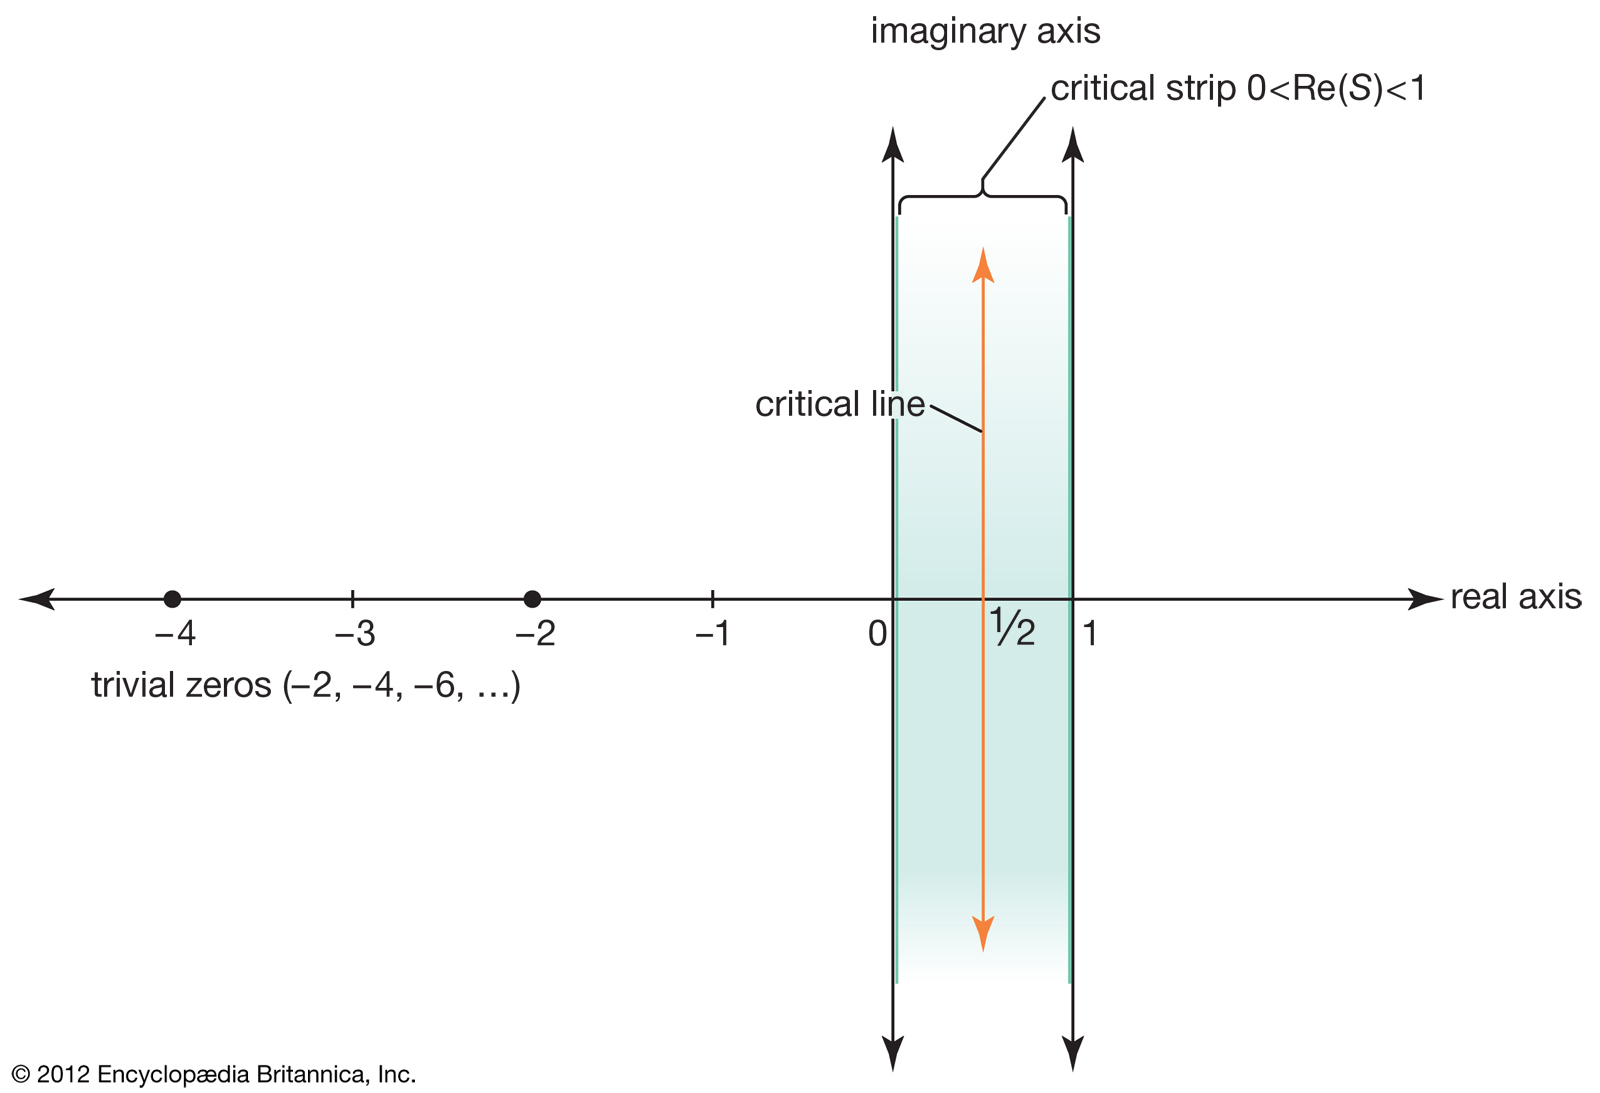
\includegraphics[width=\textwidth]{critical_strip}
\end{frame}

\begin{frame}{Intuition for Akiyama--Tanigawa conjecture}
A--T for Riemann zeta function: 
\[
	\left| \# \{p\leqslant N\} - \int_0^x \frac{t}{\log t}\, \dd t\right| = O(\sqrt N)
\]
\pause
(Equivalent to Riemann Hypothesis.)
\pause

A--T for elliptic curves implies:
\[
	\left| \sum_{p\leqslant N} f(\theta_p) \right| = O_f(N^{\frac 1 2})
\]
\pause

A--T $\Rightarrow$ RH.\pause{} 
Is the converse true?\pause{} 
No!
\end{frame}


\section{Breaking the Akiyama--Tanigawa converse}

\begin{frame}{What is needed?}
Construct a sequence $\{\theta_p\}$ such that 
\begin{enumerate}
\item<1-> Sums of the form $\sum_{p\leqslant N} f(\theta_p)$ have ``good bounds'' like $O(\sqrt N)$.
\item<2-> The discrepancy $\disc_{\{\theta_p\}}(N)$ is \emph{not} $O(N^{-\frac 1 2})$. 
\end{enumerate}
\end{frame}

\begin{frame}{Key idea}
Choose an angle $\theta$, and let let $\theta_n = n\theta \mod \pi$. Then 
\[
	\left|\sum_{n\leqslant N} e^{2\pi i m \theta_n}\right| = O\left(\frac{1}{|e^{2\pi i \theta}-1|}\right)
\]
\pause

\alert{Right-hand-side doesn't depend on $N$.}
\pause

\begin{block}{Corollary}
If $f$ is a smooth function, then 
\[
	\left|\sum_{n\leqslant N} f(\theta_n)\right| = O_f(1) .
\]
\end{block}
\end{frame}

\begin{frame}{Two degrees of freedom}
If $\theta_{p_n} = n \theta$, then 
\[
	L_f(s) = \prod_p \frac{1}{1-f(\theta_p)p^{-s}}
\]
satisfies Riemann Hypothesis. 
\pause

Also, we can control the discrepancy of the sequence $\{\theta_p\}$ via an 
\emph{irrationality exponent}.
\end{frame}

\begin{frame}{Diophantine approximation}
\begin{block}{Definition}
The \emph{irrationality exponent} of $x$ is the largest $\eta$ such that 
\[
	\left| x - \frac p q\right| < q^{-\eta}
\]
for infinitely many $p/q$. 
\end{block}
\pause

\begin{theorem}[Thue--Siegel--Roth]
If $x$ is algebraic but not rational (e.g.~$\sqrt 2$), then it has irrationality exponent $2$. 
\end{theorem}
\pause

\begin{theorem}
There are $x$ with arbitrary irrationality exponent $>2$. 
\end{theorem}
\end{frame}

\begin{frame}{Putting things together}
\begin{theorem}
For any $\eta\in (-1/2,0)$, there exists a sequence $\{\theta_p\}$ such that 
\[
	L(\{\theta_p\},s) = \prod_p \frac{1}{(1-e^{i\theta_p} p^{-s})(1-e^{-i\theta_p} p^{-s})}
\]
satisfies the Riemann Hypothesis, but for which 
\[
	\disc(N) \ne O(N^\eta) .
\]
\end{theorem}
\pause

\alert{Problem:} this sequence $\{\theta_p\}$ is uniformly distributed, not 
$\ST$-distributed. 
\end{frame}

\begin{frame}{Inverse inverse sampling transform}
If $\tilde\theta_p = \cdf_{\ST}^{-1}(\theta_p)$, then $\{\tilde\theta_p\}$ is 
$\ST$-distributed. 
\pause

Also $\cdf_{\ST}^{-1}$ preserves discrepancy of sequences. 
\pause

Tricky part: show that Riemann Hypothesis holds for $\{\tilde\theta_p\}$. 
\pause

\alert{Problem:} the $\tilde\theta_p$ don't come from integral $a_p$.
\pause

Solution: tweak them so they do, then prove everything still works. 
\end{frame}





\section{Generalizations}

\begin{frame}
From $y^2=x^3+a x+b$ to $y^2=x^5-1$:
\begin{center}
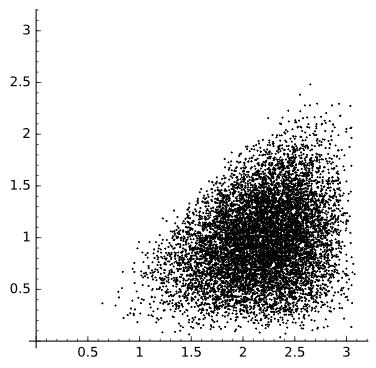
\includegraphics[width=0.6\textwidth]{genus2}
\end{center}
\pause

Higher-dimensional counterexamples.
\end{frame}

\begin{frame}
\begin{center}
{\Huge Questions?}
\end{center}
\end{frame}

\begin{frame}{Further reading}
d
\end{frame}





\end{document}
